% Redrawn from https://gregable.com/2008/11/i/q2-replacement.png
% Rebuild: latex -interaction=nonstopmode -halt-on-error pq-tree-17.tex
%          dvisvgm --no-fonts --exact-bbox --bbox=papersize pq-tree-17.dvi -o pq-tree-17.svg
\documentclass[tikz,border=4pt]{standalone}
\usetikzlibrary{backgrounds}
\pgfdeclarelayer{edges}
\pgfsetlayers{background,edges,main}
\definecolor{empty}{HTML}{D3D6DB}
\definecolor{full}{HTML}{20242B}
\definecolor{outline}{HTML}{394150}
\definecolor{edge}{HTML}{29466B}
% P nodes, Q nodes, and subtree roots are named for the edges below.
\newcommand{\pnode}[4]{%
  \node[circle,draw=outline,fill=#4,minimum size=6.8mm,inner sep=0pt]
    (#1) at (#2,#3) {};
}
% Q node: name, left, right, height, start and end of the full segment.
\newcommand{\qnode}[6]{%
  \coordinate (#1) at ({(#2+#3)/2},#4);
  \fill[empty] (#2,{#4-.19}) rectangle (#3,{#4+.19});
  \fill[full] (#5,{#4-.19}) rectangle (#6,{#4+.19});
  \draw[outline] (#2,{#4-.19}) rectangle (#3,{#4+.19});
}
\newcommand{\subtree}[4]{%
  \coordinate (#1) at (#2,#3);
  \filldraw[draw=outline,fill=#4]
    (#2,#3) -- ({#2-.38},{#3-.78}) -- ({#2+.38},{#3-.78}) -- cycle;
}
\newcommand{\siblings}[2]{%
  \foreach \dx in {-.17,0,.17}
    \fill[full] ({#1+\dx},{#2-.57}) circle[radius=.045];
}
\begin{document}
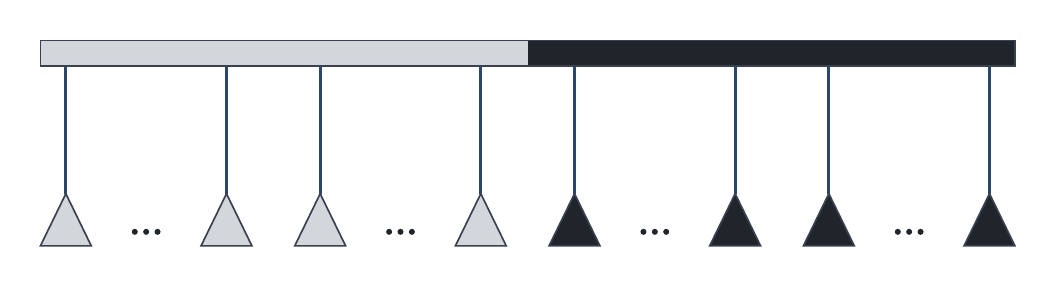
\begin{tikzpicture}[x=8.5mm,y=8.5mm,line width=.6pt,
  background rectangle/.style={fill=white},show background rectangle,
  edge/.style={draw=edge,line width=1.1pt,line cap=round}]
\qnode{u}{-0.38}{14.18}{2.1}{6.9}{14.18}
\subtree{e1}{0}{0}{empty}
\subtree{e2}{2.4}{0}{empty}
\siblings{1.2}{0}
\subtree{le1}{3.8}{0}{empty}
\subtree{le2}{6.2}{0}{empty}
\siblings{5}{0}
\subtree{lf1}{7.6}{0}{full}
\subtree{lf2}{10}{0}{full}
\siblings{8.8}{0}
\subtree{f1}{11.4}{0}{full}
\subtree{f2}{13.8}{0}{full}
\siblings{12.6}{0}
% Keep edges behind the node fills and above the white background.
\begin{pgfonlayer}{edges}
\draw[edge] (e1 |- u) -- (e1);
\draw[edge] (e2 |- u) -- (e2);
\draw[edge] (le1 |- u) -- (le1);
\draw[edge] (le2 |- u) -- (le2);
\draw[edge] (lf1 |- u) -- (lf1);
\draw[edge] (lf2 |- u) -- (lf2);
\draw[edge] (f1 |- u) -- (f1);
\draw[edge] (f2 |- u) -- (f2);
\end{pgfonlayer}
\end{tikzpicture}
\end{document}
